\chapter{CHỌN ĐỘNG CƠ ĐIỆN VÀ PHÂN BỐ TỈ SỐ TRUYỀN}
    \section{CHỌN ĐỘNG CƠ ĐIỆN}
        \subsection{Hiệu suất chung của hệ thống}
            \begin{figure}[H]
                \centering
                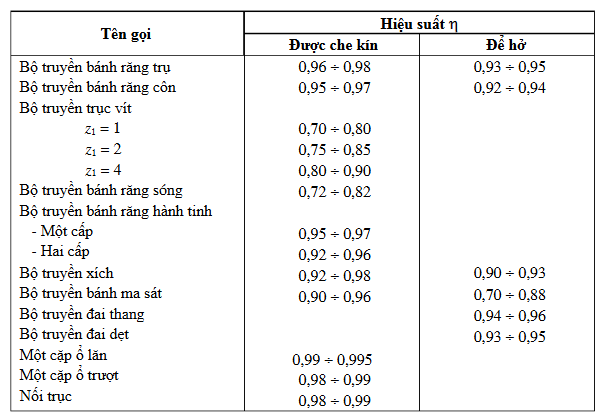
\includegraphics[width=0.8\textwidth]{pictures/table_1.png}
                \caption{Hiệu suất các bộ truyền chủ yếu}
            \end{figure}
            \hspace*{0.6cm}Dựa vào bảng hiệu suất các bộ truyền chủ yếu như trên, ta có:
            \begin{itemize}
                \item Hiệu suất của bộ truyền đai: $\eta_{d} = 0.94$.
                \item Hiệu suất của bộ truyền bánh răng trụ răng nghiêng để kín: $\eta_{br1} = 0.96$.
                \item Hiệu suất của bộ truyền bánh răng côn để hở: $\eta_{br2} = 0.92$.
                \item Hiệu suất của 2 cặp ổ lăn: $\eta_{ol}^2 = 0.99^2$.
            \end{itemize}
            \begin{center}
                $\eta_{ch}=\eta_{d} \cdot \eta_{br1} \cdot \eta_{br2} \cdot \eta_{ol}^2 = 0.94 \cdot 0.96 \cdot 0.92 \cdot 0.99^2 = 0.814 $.
            \end{center}
        \subsection{Công suất động cơ cần thiết}
            \begin{figure}[H]
                \centering
                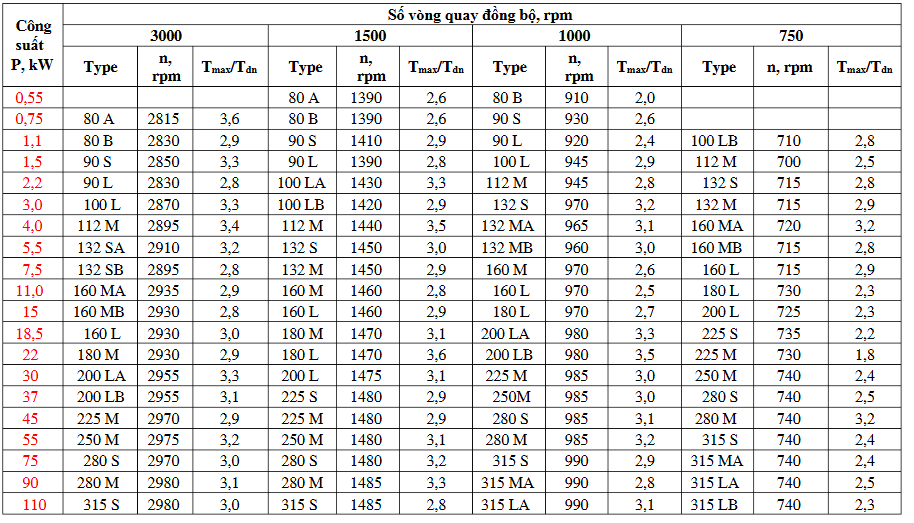
\includegraphics[width=1\textwidth]{pictures/table_2.png}
                \caption{Bảng chọn động cơ 3 pha không đồng bộ}
            \end{figure}
            \begin{center}
                $P_{dc}=\frac{P_{ct}}{\eta_{ch}} = \frac{2.5}{0.814} = 3.07 (kW)$.
            \end{center}
        \subsection{Xác định số vòng quay sơ bộ}
            \begin{figure}[H]
                \centering
                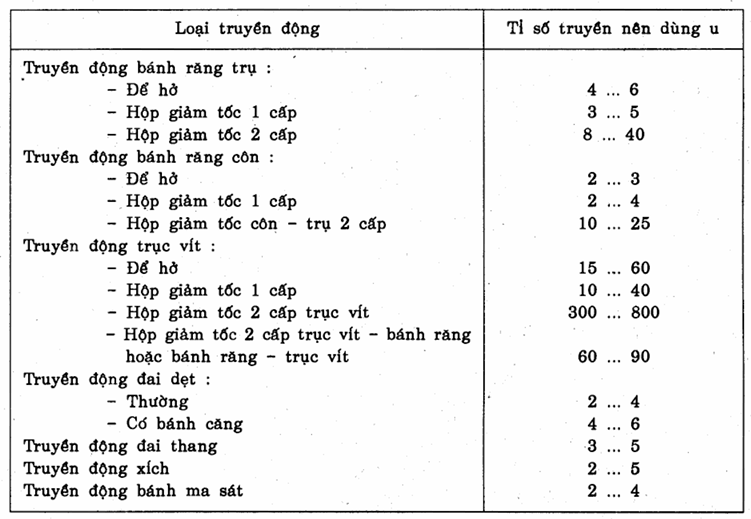
\includegraphics[width=0.8\textwidth]{pictures/table_3.png}
                \caption{Bảng chọn tỉ số truyền}
            \end{figure}
            \begin{itemize}
                \item Chọn tỉ số truyền \footnote{Tra bảng [2.4], tài liệu tham khảo \cite{tltk1} }: $u_{br1} = 5; u_{br2} = 6; u_{d} = 2$\\
                \item Tỷ số truyền hệ thống: $u_{ch}=u_{br1} \cdot u_{br2} \cdot u_{d}=\frac{n_{dc}}{n_{ct}} = 6 \cdot 5 \cdot 2 = 60$.\\
                \item Số vòng quay sơ bộ của động cơ: $n_{sb} = n_{ct} \cdot u_{ch} = 12 \cdot 60 = 720.$
            \end{itemize}
        \subsection{Chọn động cơ}
            \hspace*{0.6cm}Dựa vào bảng chọn Động cơ 3 pha Không đồng bộ, chọn lấy động cơ có công suất lớn hơn 3.07(kW) và gần nhất. Từ đó, ta có động cơ công suất 4(kW).\\
            \begin{table}[H]
                \centering
                \begin{tabular}{|>{\centering\arraybackslash}m{1.8cm}|>{\centering\arraybackslash}m{2.5cm}|>{\centering\arraybackslash}m{2.5cm}|>{\centering\arraybackslash}m{2.5cm}|>{\centering\arraybackslash}m{2.5cm}|>{\centering\arraybackslash}m{2.5cm}|}
                    \hline
                    \textbf{Động cơ} & \textbf{Số vòng quay động cơ $n_{dc}$ (vg/ph)} & \textbf{Tỷ số truyền chung $u_{ch}$} & \textbf{Bộ truyền đai thang} & \textbf{Bộ truyền bánh răng trụ kín $u_{br1}$} & \textbf{Bộ truyền bánh răng côn hở $u_{br2}$} \\ 
                    \hline
                    ĐC1 & 2895 & 241.25 & 2 & 12.5 & 9.65 \\
                    \hline
                    ĐC2 & 1440 & 120 & 2 & 11.2 & 5.36 \\
                    \hline
                    ĐC3 & 965 & 80.42 & 2 & 8 & 5.03 \\ 
                    \hline
                    ĐC4 & 720 & 60 & 1.5 & 8 & 5 \\
                    \hline 
                \end{tabular}
                \caption{Động cơ và phân phối tỉ số truyền}
                \label{tab:gear_ratios}
            \end{table}
            \hspace*{0.6cm}Chọn động cơ sao cho thỏa mản $P_{dc} > =P{ct}$ và $n_{dc} \approx n_{sb}$, ta chọn động cơ 4 (Động cơ 160MA).\\
            \hspace*{1.2cm}Động cơ 4: $P_{dc} = 4.0(kW); n_{dc} = 720(vg/ph); u_{ch} = 60; u_{br1} = 8; u_{br2} = 5; u_{d} = 1.5$.
    \section{PHÂN PHỐI TỈ SỐ TRUYỀN}
        \subsection{Công suất trên từng trục}
            \begin{itemize}
                \item $P_{III} = \frac{P_{ct}}{\eta_{br2}} = \frac{2.5}{0.92} = 2.72(kW)$.
                \item $P_{II} = \frac{P_{III}}{\eta_{br1}.\eta{ol}} = \frac{2.72}{0.96.0.99} = 2.86(kW)$.
                \item $P_{I} = \frac{P_{II}}{\eta_{d}.\eta{ol}} = \frac{2.86}{0.94.0.99} = 3.07(kW)$.
            \end{itemize}
        \subsection{Số vòng quay trên từng trục}
            \begin{itemize}
                \item $n_{II} = \frac{n_{dc}}{u_{d}} = \frac{720}{2} = 360$ (vg/ph). 
                \item $n_{III} = \frac{n_{II}}{u_{br1}} = \frac{360}{5} = 72$ (vg/ph).
                \item $n_{IV} = \frac{n_{III}}{u_{br2}} = \frac{72}{6} = $ (vg/ph).
            \end{itemize}
        \subsection{Moment xoắn trên trục}
            \begin{itemize}
                \item $T_{I} = 9.55.10^3.\frac{P_{I}}{n_{I}} = 9.55.10^3.\frac{3.07}{720} = 40.72(N.m).$
                \item $T_{II} = 9.55.10^3.\frac{P_{II}}{n_{II}} = 9.55.10^3.\frac{2.86}{360} = 75.87(N.m).$
                \item $T_{III} = 9.55.10^3.\frac{P_{III}}{n_{III}} = 9.55.10^3.\frac{2.72}{72} = 360.78(N.m).$
                \item $T_{IV} = 9.55.10^3.\frac{P_{IV}}{n_{IV}} = 9.55.10^3.\frac{2.5}{12} = 1989.58(N.m).$
            \end{itemize}
            \begin{table}[H]
                \centering
                \begin{tabular}{|>{\centering\arraybackslash}m{4.2cm}|>{\centering\arraybackslash}m{2.5cm}|>{\centering\arraybackslash}m{2.5cm}|>{\centering\arraybackslash}m{2.5cm}|>{\centering\arraybackslash}m{2.5cm}|}
                    \hline
                    \diagbox{\textbf{Thông số}}{\textbf{Trục}} & \textbf{I} & \textbf{II} & \textbf{III} & \textbf{IV} \\ 
                    \hline
                    Công suất (kW) & 3.07 & 2.86 & 2.72 & 2.5 \\
                    \hline
                    Tỷ số truyền & \multicolumn{1}{c|}{2} & \multicolumn{2}{c|}{5} & \multicolumn{1}{c|}{6}\\
                    \hline
                    Momen xoắn (N.m) & 40.72 & 75.87 & 360.78 & 1989.58 \\ 
                    \hline
                    Số vòng quay (vòng/ph) & 720 & 360 & 72 & 12 \\
                    \hline 
                \end{tabular}
                \caption{Đặc tính kỹ thuật hệ thống truyền động}
                \label{tab:technical_specifications}
            \end{table}